\subsection{Reverberation}\label{sec:reverberation} 
\gls{reverb} is an effect where a sound wave is reflected, and therefore those waves have another travelling time and amplitude than the initial sound directly from the source, when they arrive to the listener. This effect is very frequent; it happens each time a sound is reflected by walls, trees, tables and other surfaces which reflect sound. The following \autoref{fig:reverb_reflect} shows the \gls{reverb} effect waves paths from one person, the sound source, to another, the listener \citep{reverb_expl}.

\begin{figure} [htbp]
 \centering
\begin{picture}(0,0)%
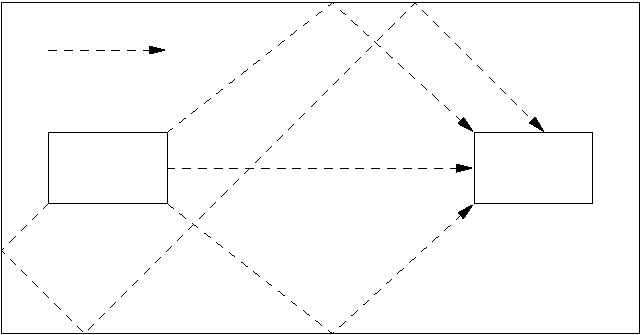
\includegraphics{reverb_reflect.pdf}%
\end{picture}%
\setlength{\unitlength}{4144sp}%
%
\begingroup\makeatletter\ifx\SetFigFont\undefined%
\gdef\SetFigFont#1#2#3#4#5{%
  \reset@font\fontsize{#1}{#2pt}%
  \fontfamily{#3}\fontseries{#4}\fontshape{#5}%
  \selectfont}%
\fi\endgroup%
\begin{picture}(4884,2544)(2329,-3313)
\put(2746,-1006){Sound wave}%
\put(2746,-2086){$Source$}%
\put(6031,-2086){$Listener$}%
\end{picture}%
  \caption{The path of the \gls{reverb} effects sound waves.}
  \label{fig:reverb_reflect}
\end{figure}

The received reflected sound is actually a mix of very fast echoes, a merge with all the reflected sounds and the direct one, so the effect is noticed as a single sound, although it may be more than 100 echoes. 
\gls{reverb} makes a complex mix of echoes which brings depth to the guitar sound, and makes it more natural \citep{reverb_natural}.

A simple block diagram of the \gls{reverb} effect is shown at \autoref{fig:reverb_block}.

\begin{figure} [htbp]
 \centering
\begin{picture}(0,0)%
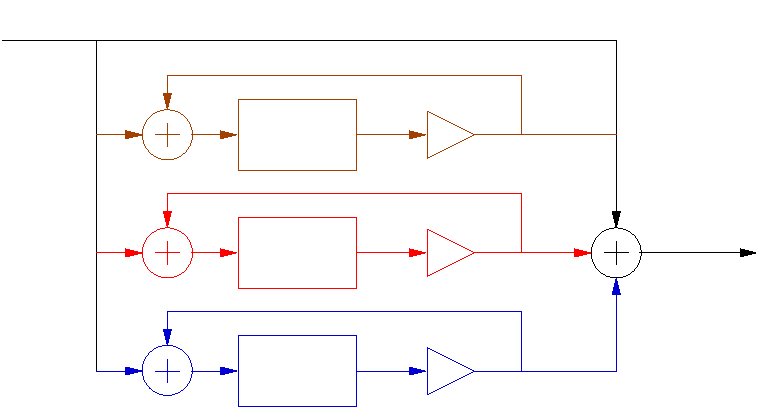
\includegraphics{reverb.pdf}%
\end{picture}%
\setlength{\unitlength}{4144sp}%
%
\begingroup\makeatletter\ifx\SetFigFont\undefined%
\gdef\SetFigFont#1#2#3#4#5{%
  \reset@font\fontsize{#1}{#2pt}%
  \fontfamily{#3}\fontseries{#4}\fontshape{#5}%
  \selectfont}%
\fi\endgroup%
\begin{picture}(5787,3120)(886,-1603)
\put(5493,-512){\makebox(0,0)[lb]{\smash{{\SetFigFont{20}{24.0}{\rmdefault}{\mddefault}{\updefault}{\color[rgb]{0,0,0}+}%
}}}}
\put(2791,1334){$Main$}%
\put(901,1334){$Input$}%
\put(5896,-286){$Output$}%
\put(4321,704){\color[rgb]{.63,.25,0}$Gain$}%
\put(2791,434){\color[rgb]{.63,.25,0}$Delay$}%
\put(2791,-466){\color[rgb]{0,0,1}$Delay$}%
\put(4321,-241){\color[rgb]{0,0,1}$Gain$}%
\put(4321,-1141){\color[rgb]{1,0,0}$Gain$}%
\put(2791,-1366){\color[rgb]{1,0,0}$Delay$}%
\put(2071,389){\makebox(0,0)[lb]{\smash{{\SetFigFont{20}{24.0}{\rmdefault}{\mddefault}{\updefault}{\color[rgb]{.63,.25,0}+}%
}}}}
\put(2071,-512){\makebox(0,0)[lb]{\smash{{\SetFigFont{20}{24.0}{\rmdefault}{\mddefault}{\updefault}{\color[rgb]{0,0,1}+}%
}}}}
\put(2072,-1412){\makebox(0,0)[lb]{\smash{{\SetFigFont{20}{24.0}{\rmdefault}{\mddefault}{\updefault}{\color[rgb]{1,0,0}+}%
}}}}
\end{picture}%
  \caption{The figure shows a block diagram of a \gls{reverb} unit.}
  \label{fig:reverb_block}
\end{figure}

The block diagram \autoref{fig:reverb_block} shows the direct sound path and only a few delay blocks with their individual gain and delay. Normally, there are many more delay lines. All signals are added together just before the output line. A time domain diagram is shown in \autoref{fig:reverb_timed}. Each colour refers to \autoref{fig:reverb_block} and is just an example of an impulse response. With other settings at gain and delay, the impulse response will look different.


\begin{figure} [htbp]
 \centering
\begin{picture}(0,0)%
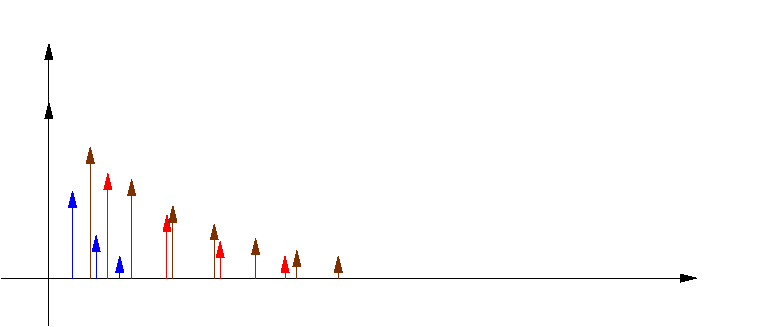
\includegraphics{reverb_timed.pdf}%
\end{picture}%
\setlength{\unitlength}{4144sp}%
%
\begingroup\makeatletter\ifx\SetFigFont\undefined%
\gdef\SetFigFont#1#2#3#4#5{%
  \reset@font\fontsize{#1}{#2pt}%
  \fontfamily{#3}\fontseries{#4}\fontshape{#5}%
  \selectfont}%
\fi\endgroup%
\begin{picture}(5843,2478)(4129,-5833)
\put(9496,-5506){$Time$}%
\put(4231,-3526){$Magnitude$}%
\put(4591,-4291){$Main$}%
\end{picture}%
  \caption{Impulse response of a \gls{reverb} unit.}
  \label{fig:reverb_timed}
\end{figure}

